\chapter{Algorithm}\label{cp:algo}

This chapter explains the general principles behind the algorithm and separates the logic from the implementation, which will be discussed in a separate chapter, \nameref{cp:sw}. 

The realised algorithm is a fixed-ratio algorithm. It analyses the oscillations to find MAP form the maximum amplitude as described in \myref{sec:MAA} and estimates the position of the systolic and diastolic BP as where the amplitudes are at a specific ratio of the maximum. The systolic BP is evaluated while the oscillation amplitudes increase and the diastolic BP while they decrease, respectively.


\begin{figure}[ht]
\centering
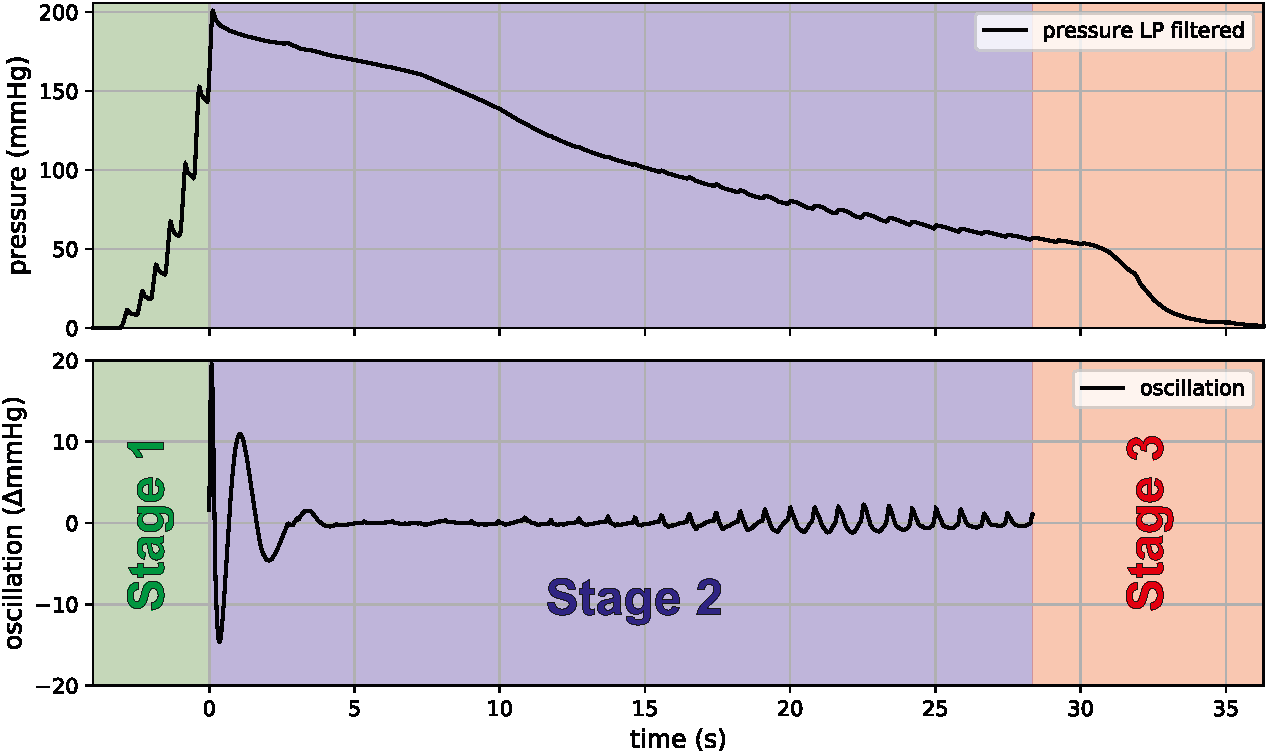
\includegraphics[width=\textwidth]{figures/algo_overview.pdf}
\caption{A sample data set is shown in the top plot and divided into three parts. The blue part is where oscillations are analysed. These are shown in the bottom plot.}
\label{fig:algoOverview}
\end{figure}

The top plot in figure \ref{fig:algoOverview} shows one data set and how it is divided into different steps for processing. The first part (green) is when the user pumps up the cuff pressure. The second part (blue) is the deflation. Here, the oscillations, shown in the bottom plot, are recorded and analysed. Once these oscillations have increased to a maximum and decreased again to a certain value, the last step (red) is simply the deflation of the cuff. The core part of the algorithm works on the blue part of the data.



\section{Preprocessing}
The data is always filtered. Additionally, preprocessing decides which stage of the dataset is active. In relation to figure \ref{fig:algoOverview} stage one is green, stage two is blue and stage three is red. Figure \ref{fig:stage1} shows the basic diagram of the data processing. Only the deflating and filtered data is processed by the core algorithm. 

\subsection{Filtering}\label{sec:filt}
To remove unwanted noise from the data and to get the oscillations, two filters are used. Figure \ref{fig:stage1} shows the simple cascade of a low-pass (LP) and high-pass (HP) filter, resulting in a bandpass(BP) filtered output signal, the oscillogram. The results of both filter outputs are used in the algorithm.
%
%\begin{figure}[ht]
%\centering
%\includegraphics[width=0.7\textwidth]{figures/filter_cascade.pdf}
%\caption{The simple basic data processing flow. The data is acquired and passed first to a low-pass filter \SI{10}{\Hz} and then to a high-pass filter of \SI{0.5}{\Hz}, resulting in a bandpass output.}
%\label{fig:filter_cascade}
%\end{figure}

\begin{figure}[ht]
\centering
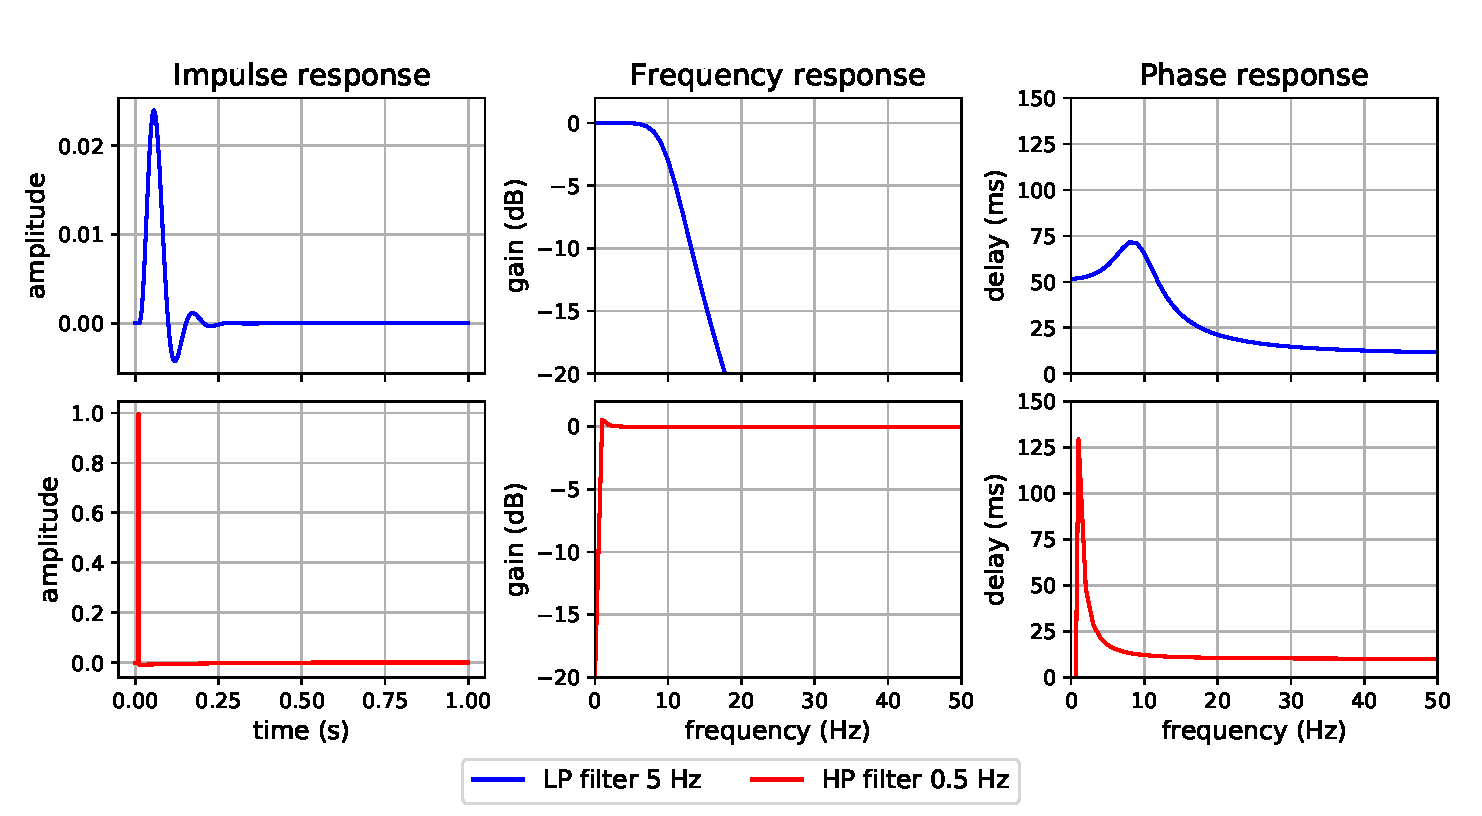
\includegraphics[width=\textwidth]{figures/filter.pdf}
\caption{Filter.}
\label{fig:filters}
\end{figure}
%All data is filtered. 

From the research done in chapter \ref{cp:theory}, it is known that most algorithms use band pass filters of low orders up to \nth{6} and with cut-off frequencies between \SIrange{0.1}{0.5}{\Hz} and \SIrange{5}{20}{\Hz} \citep{Forouzanfar2015}. The implemented algorithm does not rely on pulse shape and can therefore use relaxed constraints. Best results were achieved with a lower cut-off frequency of \SI{0.5}{\Hz}. The upper cut-off frequency was fixed \SI{10}{\Hz}. Generally, there is very little activity between \SIrange{5}{20}{\Hz}, but because no experiments could be made, a mean value was chosen. 

The implemented filters are shown in figure \ref{fig:filters}. The low-pass filter has a small delay in the impulse response and the phase response shows that for very low frequencies there is a slightly higher delay. The frequency response shows a steep slope after \SI{10}{\Hz} and suppression of more than \SI{20}{\decibel} of every frequency above \SI{20}{\Hz}. The HP filter expectedly lets the impulse pass. In the frequency response there is a small overshoot but otherwise a good suppression of DC. The bottom left plot in figure \ref{fig:filters} shows that HP filter has a significantly delay of about \SI{125}{\milli\second} for frequencies around \SI{1}{\Hz}. This could potentially cause inaccuracies. Section \ref{sec:impfilt} will show, why this is not a problem.


%TODO referecne section


\subsection{Stage Detection}
The LP filtered data is analysed by the preprocessing step to detect if the second stage, the deflation, is active. Figure \ref{fig:stage1} shows how the preprocessing step then passes both the LP and BP filtered data to the core algorithm, symbolised by a switch. 

In the first stage, the data is checked if the pressure in the cuff is high enough to start deflation and if so, the preprocessing switches to the second stage. This value is configurable. The default value is \SI{180}{\mmHg}. Figure \ref{fig:stage1} shows how the decision is made based on the LP filtered data.  

Once the second stage is active, the preprocessing checks the core algorithm if it is done. In figure \ref{fig:stage1} this is indicated by the arrow from the algorithm back to preprocessing. Additionally, the data is checked if it is below a value of \SI{20}{\mmHg}, where blood pressure measurements make no sense, and the measurement is  potentially cancelled.

\begin{figure}[ht]
\centering
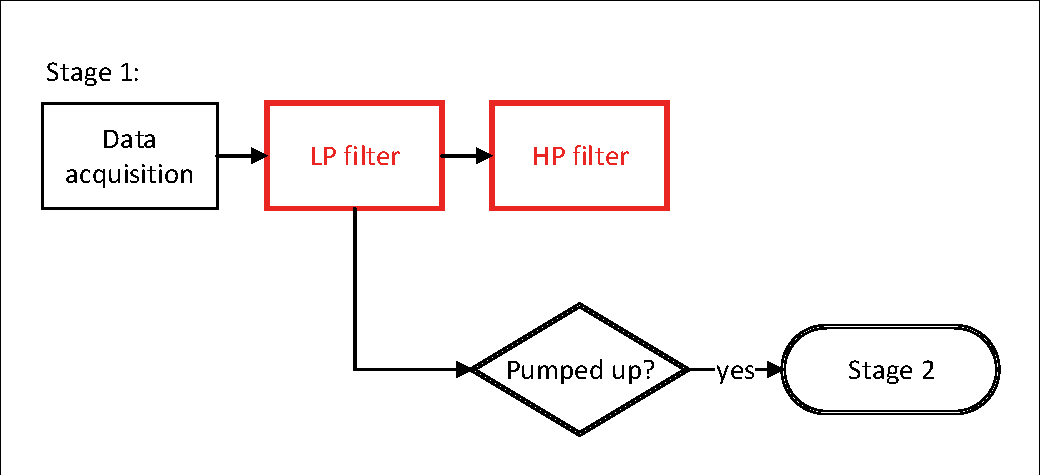
\includegraphics[width=0.7\textwidth]{figures/stage1.pdf}
\caption{The simple basic data processing flow. The data is acquired and passed first to a low-pass filter (\SI{10}{\Hz}) and then to a high-pass filter (\SI{0.5}{\Hz}), resulting in a bandpass output. The first stage of the data processing only checks, if the pressure in the cuff is high enough to start deflation (stage 2).}
\label{fig:stage1}
\end{figure}

\section{Deflation}\label{sec:Deflation}
Figure \ref{fig:algoExplain} shows data recorded during the deflation stage. \circled{1} shows the low pass filtered data which is used in the core algorithm as a reference. \circled{2} is the BP filtered data upon which the algorithm is performed. 

\begin{figure}[ht]
\centering
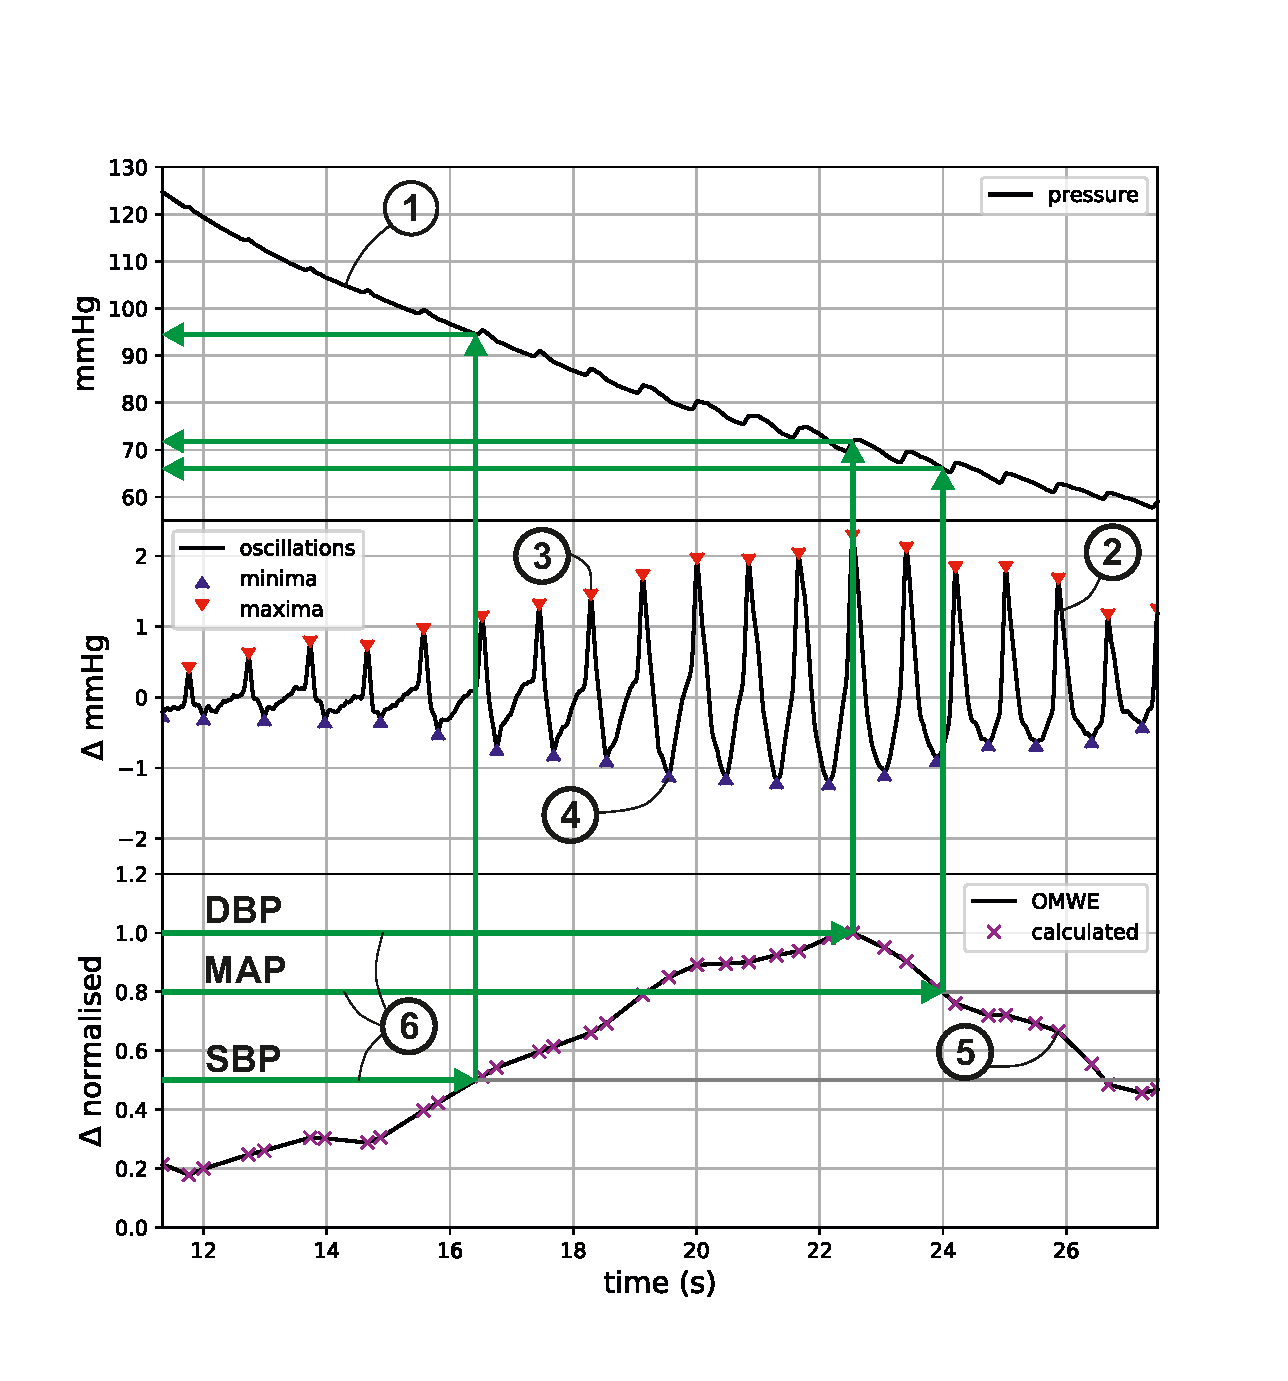
\includegraphics[width=0.95\textwidth]{figures/algorithm_example_annotated.pdf}
\caption{Algo explanation.}
\label{fig:algoExplain}
\end{figure}



\subsection{Extrema Detection}
\paragraph{Maxima}The next step, indicated with \circled{3} is to detect the maxima. Looking at the oscillations, there are local maxima in the troughs between two oscillations. To avoid detecting these, a value needs to have a minimal pronunciation of \SI{0.25}{\Delta\mmHg} to even be considered as a maxima. This limits how the quickly the first oscillations can be detected, but does not influence the algorithm because they are less than \SI{10}{\percent} of the expected maximal amplitude.

A sample is identified as a local maxima, due to the previous and following value being lower. Next, is checked if the current and last detected maxima result in a valid heart rate given by a configurable range. The default range is \SIrange{50}{100}{beats/\minute}. In addition, if the last maxima was less than \SI{300}{\milli\second} ago, only the larger of the two is kept and the lower is discarded.

This is due to two factors that were observed in the data and are shown if figure \ref{fig:maxDetectIssue}. The first, shown on the left hand side, is if the bump in the rising edge of the oscillations results in a detected maxima. This is likely due to artefacts from movement. When oscillations are small and rising, these can lead to wrong detections. This is either irrelevant because they occur before systolic BP or they will be discarded because they lead to errors. 

The second issue is shown in figure \ref{fig:maxDetectIssue} on the right. It occurs mainly when oscillations are decreasing and if the filtering is not optimal. 
\paragraph{Minima} Minima detection, indicated by \circled{4} in figure \ref{fig:algoExplain}, is considerably more difficult, especially in the beginning of oscillations as shown in figure \ref{fig:oscMini}. Because there has to be a minima in between two maxima, minima detection is simplified. After detecting two maxima, the lowest value between them is recorded as the minima.


\subsection{Heart Rate Detection}\label{sec:HR}
Heart rate is already part of the extrema detection described above. Therefore, the current heart rate is detected after each valid maxima starting from the second one. Because each pulse stems from a heart beat, each maxima represents one. By calculating the time between the last two maxima, a heart beat is estimated using equation \ref{eq:HR} below.

\begin{equation}
\label{eq:HR}
pulse=\frac{60s}{t_{curMax} - t_{lastMax}}
\end{equation}

After finishing the measurement, the average heart rate is calculated from all validly detected maxima.


\section{Oscillometric Waveform Envelope}
When the detected maxima, marked by the red triangles in \ref{fig:algoExplain}, have reached their highest amplitude and declined again the oscillometric waveform envelope (OMWE) can be calculated. 

This condition is estimated by taking the largest recorded maximum and multiplying it with the ratio for the diastolic blood pressure minus a hysteresis of $0.3$ (equation \ref{eq:cutoff}. If the last recorded maxima is below this value, the extrema detection part of the algorithm (\circled{3} and \circled{4} in figure \ref{fig:algoExplain}) can be concluded. To avoid a wrong detection of this condition the largest maxima needs to be at least \SI{1.5}{\delta\mmHg}. Otherwise the condition can be detected when oscillations first start occurring and are small with large variations. 

\begin{equation}
\label{eq:cutoff}
A_{cutoff}=A_{Max}\times (r_{DBP} - 0.3)
\end{equation}

\subsection{OMWE Calculation}
To calculate the OMWE from the determined extrema, the following approaches were tested:

\begin{enumerate}[noitemsep]
\item Only considering the maxima.
\item Subtracting the following minimum from each maxima.
\item Subtracting the preceding minimum from each maxima.
\item Interpolating between maxima and minima to find the corresponding values and subtracting them. 
\end{enumerate}

1. works decently, but discards the information in the minima. 2. works well for pressure in the systolic range, because minima follow quickly after maxima. Vice versa, 3. works well in the diastolic range. 4. requires the most computations, but is the least sensitive to noise, because it takes the time difference between minima and maxima into consideration. 

When referring back to figure \ref{fig:algoExplain}, \circled{5} shows how the OMWE was calculated using the \nth{4}approach and calculating a value for each of the maxima and minima separately. 

Figure \ref{fig:interpol} shows how interpolation is used to calculate an interpolated maximum at the time where a minimum occurs to then be able to subtract the minimum from the maximum. Inversely, A minimum is interpolated between two measured minima where a maximum occurs. The resulting plot is displayed in figure \ref{fig:algoExplain} at the bottom. Note that the values are normalised by the maximal value.


\subsection{Determination of Blood Pressure Values}
After calculating the OMWE, the last step is to determine the BP values from it. As explained in chapter \myref{cp:theory}, MAP occurs where the OMWE has its maximum. The time, when the maximum is recorded, is compared to the pressure at that time as indicated by \circled{6} in figure \ref{fig:algoExplain}. To account for the oscillations in the deflation curve, the pressure value is averaged over the period of an average heart beat centred around the detected time. The average heart beat is determined from the measurement as explained in section \myref{sec:HR}. In the example above, this results in MAP of \SI{71}{\mmHg}.

Likewise, to determine SBP and DBP, the specific ratios of the maximal oscillations are searched in the OMWE. The example in figure \ref{fig:algoExplain} uses a ratio for systolic BP of 0.5 and for diastolic BP of 0.8 for simplicity.

The systolic BP is determined by stepping backwards in time from the maximal oscillations and the diastolic BP by stepping forwards in time, respectively. Once the value falls below the specific ratio, interpolation is used to find the time where the exact ratio would have occurred. Using the same approach as for the MAP, the specific values found with \circled{6} for the data in figure \ref{fig:algoExplain} is \SI{95}{\mmHg} for SBP and \SI{67}{\mmHg} for DBP.

%TODO results?
\subsubsection{Implications of Filter Delays}\label{sec:impfilt}
As pointed out in section \myref{sec:filt}, the original data is delayed by first the LP and then the HP filter. Since the oscillogram is based on the LP filtered data, the delay of the first filter (LP) is irrelevant. The second filter (HP) has up to \SI{125}{\milli\second} delay for certain frequencies. Figure \ref{fig:algoDetail} shows the oscillations superimposed over the deflating data. At a deflation rate of \SI{3}{\mmHg/\second}, the error could be \SI{0.375}{\mmHg}. The calculated pressure is averaged over the period of an average heart rate to account for the oscillations in the deflating data and compared to the inaccuracies of the algorithm in general, this is neglectable. 


\begin{figure}[ht]
\centering
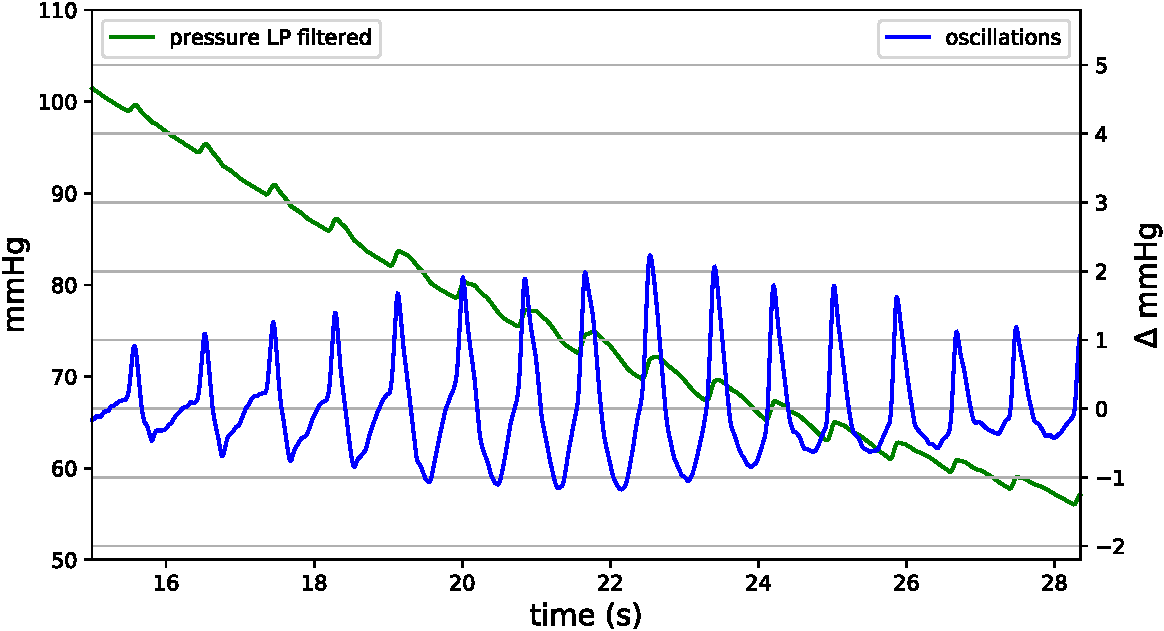
\includegraphics[width=\textwidth]{figures/algo_detail.pdf}
\caption{Algo explanation.}
\label{fig:algoDetail}
\end{figure}
